\subsection{{\bf RQ2. Comparative Study on Java Dataset}}






\subsubsection{General Results}

Table~\ref{RQ2-result-1} shows $Accuracy^{c}$ when it was measured on
the changed statements for Java code.  As seen, on the Java dataset,
{\tool} improves Base-1, Base-2, Base-3, and SmartCommit in overall
$Accuracy^c$ by {\bf 100.0\%, 36.0\%, 47.8\%}, and {\bf 13.3\%},
respectively. {\tool}'s accuracies are consistently better than those
of the baselines for all subject projects. Figure~\ref{RQ2-result-2}
shows the boxplot for $Accuracy^c$ result in
Table~\ref{RQ2-result-1}. As seen, the median accuracy of {\tool} is
higher than those of the baselines.

%Barnett {\em et al.}, Herzig {\em et al.}, $\sigma-$PDG+CV, and
%Flexeme in overall $Accuracy^c$ by {\bf 462.5\%, 55.2\%, 28.6\%}, and
%{\bf 36.4\%}, respectively. As seen in Table~\ref{RQ1-result-2}, when
%$Accuracy^{a}$ is measured on all the statements (changed and
%un-changed) in a commit, the results for all models are higher
%because they have correct classifications for the changed statements
%by default. We include $Accuracy^{a}$ for the comparison purpose with
%Flexeme (as its authors used this metric in their paper). As seen,
%{\tool} also improves Barnett {\em et al.}, Herzig {\em et al.},
%$\sigma-$PDG+CV, and Flexeme by {\bf 641.7\%, 27.1\%, 9.9\%,} and
%{\bf 7.3\%} in overall $Accuracy^{a}$, respectively.  {\tool}'s
%accuracies are consistently better than those of the baselines for
%all the projects w.r.t.~different numbers of concerns in a commit
%($\#C$s=2,3, all, Table~\ref{RQ1-result-1}). Some data points are
%unavailable since those commits are older in the chronological order
%and appear in the training, but not in the testing.

%Figure~\ref{RQ1-result-3} shows the boxplots for both $Accuracy^c$ and
%$Accuracy^a$ results in Tables~\ref{RQ1-result-1}
%and~\ref{RQ1-result-2}. The orange boxes are for the commits with two
%concerns, while the yellow ones are for those with three concerns. As
%seen, the median accuracy of {\tool} is higher than those of all
%baselines on both types of two and three concerns. Moreover, the gap
%(in \%) between {\tool} and the baselines in $Accuracy^{c}$ is larger
%than the gap between them in $Accuracy^{a}$ because all models have
%correct classifications by default for the changed statements, which
%are many more than the changed ones.

%{\color{red}{ 1--22 changed statements: 37\%--45\%. Lowest: 24\%
	
%{100\% correct: \tool: 116, SmartCommit: 109, Overlapping: 21}}

\begin{table}[t]
	\caption{RQ2. Comparison on Java Dataset ($Accuracy^c$\%)}
	\vspace{-12pt}
	\begin{center}
		\small
		\tabcolsep 4pt
		\renewcommand{\arraystretch}{1} \begin{tabular}{p{0.5cm}<{\centering}|p{1.2cm}<{\centering}|p{1.2cm}<{\centering}|p{1.2cm}<{\centering}|p{1.2cm}<{\centering}|p{1.2cm}<{\centering}}
			
			\hline
			          & Base-1 & Base-2  & Base-3 & SmartCommit & \bf {\tool}\\
			\hline
			SB   & 14 & 23 & 21 & 29 & 32\\
			ES   & 19 & 22 & 27 & 34 & 36\\
			RJ   & 18 & 28 & 24 & 31 & 33\\
			GU   & 21 & 31 & 25 & 33 & 37\\
			RE   & 22 & 24 & 19 & 29 & 34\\
			DU   & 15 & 19 & 18 & 24 & 29\\
			GH   & 22 & 27 & 24 & 33 & 35\\
			ZX   & 21 & 29 & 20 & 34 & 38\\
			DR   & 17 & 29 & 18 & 32 & 34\\
			EB   & 13 & 22 & 21 & 27 & 31\\
			\hline
			OA   &  17  & 25 &  23 & 30 & {\bf 34} \\
			\hline
		\end{tabular}
		\label{RQ2-result-1}
	SB: spring-boot, ES: elasticsearch, RJ: RxJava, GU:guava, RE: retrofit, DU: dubbo, GH: ghidra, ZX: zxing, DR: druid, EB: EventBus, OA: Overall
	\end{center}
\end{table}

\begin{figure}[t]
	\centering 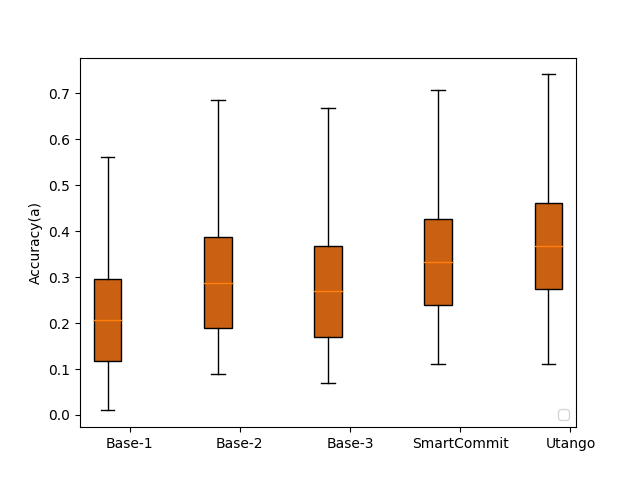
\includegraphics[width=2.2in]{figures/RQ_2_1.png}
	\vspace{-6pt}
	\caption{Boxplots for Results in Table~\ref{RQ2-result-1}}
	\label{RQ2-result-2}
\end{figure}

\begin{figure}[t]
	\centering 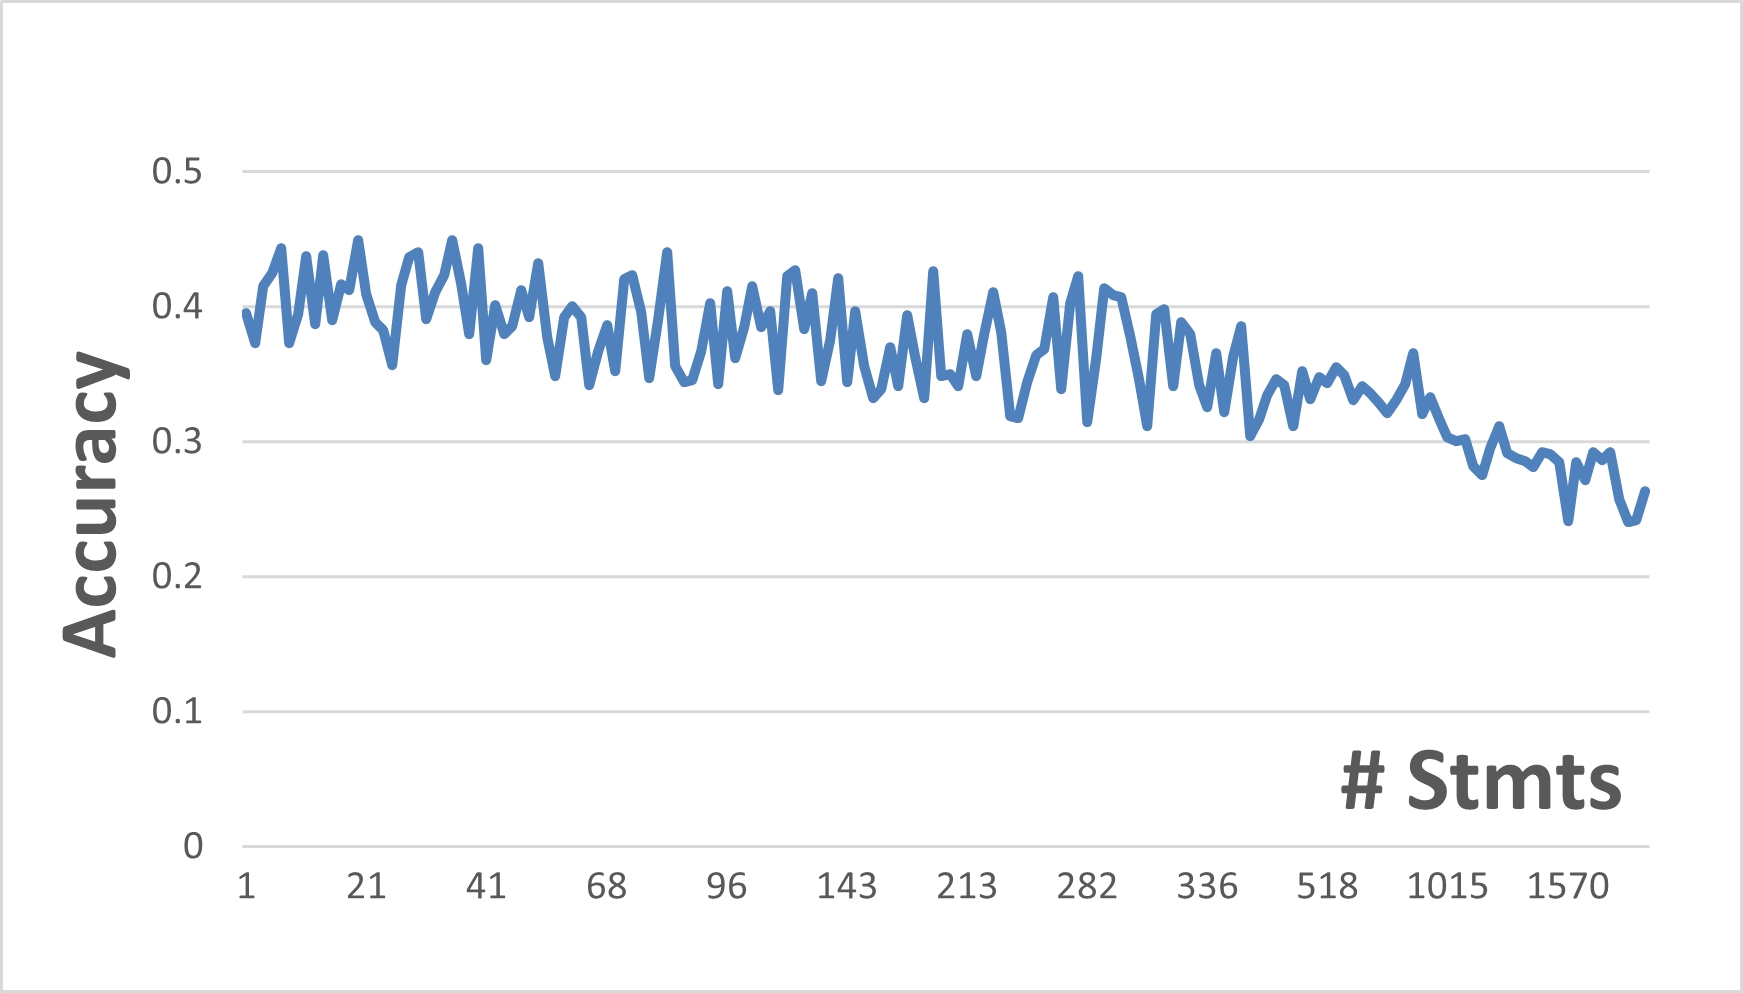
\includegraphics[width=2.4in]{figures/accuracy-concerns-java.png}
	\vspace{-6pt}
	\caption{Accuracies for Concerns with Different Numbers of Statements in Java dataset}
	\label{RQ2-result-3}
\end{figure}

%\begin{figure}
%  \centering
%  \vspace{-12pt}
%	\begin{subfigure}{0.235\textwidth}
%	\centering
%	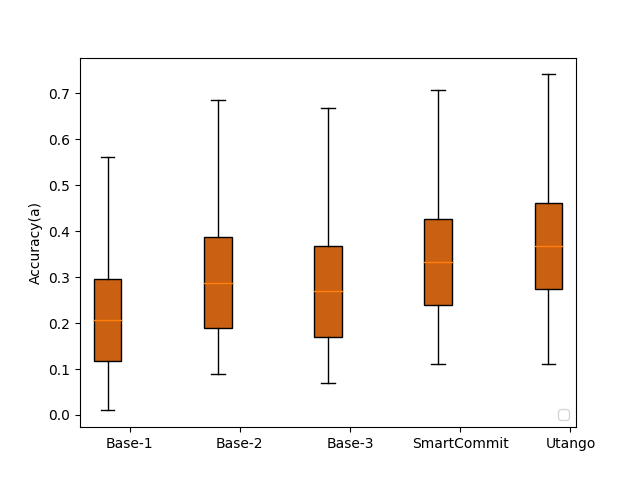
\includegraphics[width=1.6in]{figures/RQ_2_1.png}
%	\vspace{-8pt}
%	\caption{Boxplots for Results in Table~\ref{RQ2-result-1}}
%	\label{RQ2-result-2}
%	\end{subfigure}
%\hfill
%	\begin{subfigure}{0.225\textwidth}
%		\centering
%		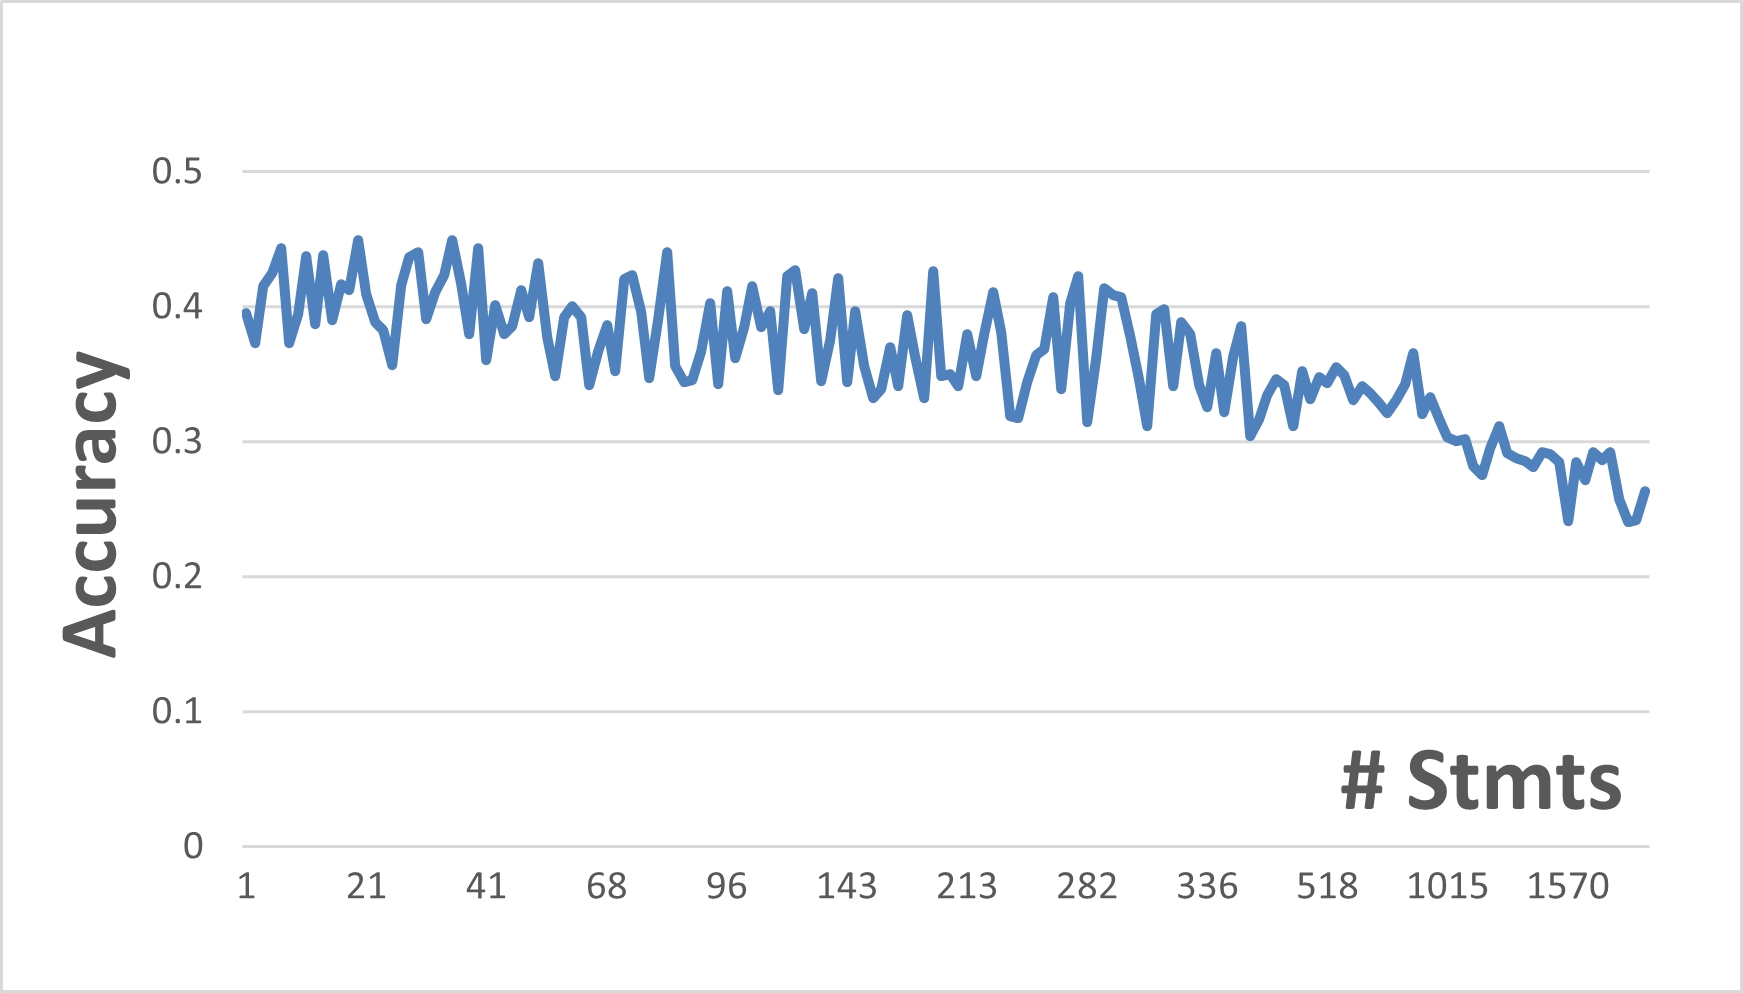
\includegraphics[width=1.7in]{figures/accuracy-concerns-java.png}
%		\vspace{-8pt}
%		\caption{Accuracy for Concern's Sizes}
%		\label{RQ2-result-3}
%	\end{subfigure}
%	\label{RQ2-result-4}
%	\vspace{-12pt}
%	\caption{Comparison and Accuracy w.r.t. Concern's Sizes}
%\end{figure}




%\vspace{2pt}
%\noindent {\bf Accuracy on Different Sizes of Concerns.}

\subsubsection{Accuracy Results for Concerns with Different Sizes}

As seen in Figure~\ref{RQ2-result-3}, $Accuracy^{c}$ values for the
concerns of smaller sizes (having 1--22 changed statements) are higher
(ranging from 37\%--45\%). That is, among all the changed statements,
{\tool} correctly classified 41\% of them into the correct clusters.
For larger concerns, $Accuracy^{c}$ decreases gradually. Even in the
concerns with up to 336 changed statements, $Accuracy^{c}$ is
$>=$30\%. The lowest accuracy is 24\%. Moreover, it
correctly classified {\em 100\% of all the changed statements} for 95
commits in which SmartCommit failed to reach 100\%. There are 88
commits that SmartCommit correctly classified all the changed
statements and {\tool} did not reach 100\%. Both~models correctly
classified 100\% of all changed statements of 21 commits.

%because it is more challenging to get correct classifications for more
%changed statements in a concern. However, $Accuracy^{c}$ decreases
%gradually with the lowest value of $\approx$ 36\%. Note: there are a
%few commits with the addition of large files of $+$1.3k lines.

Training of \tool on $80\%$ of the Java dataset takes 17 hours and
predicting on $10\%$ of Java dataset takes 1.5-4.2 seconds per commit.
Note: the Java dataset is much larger than the C\# dataset.
